\section{电磁感应}\label{sec:10-12}

丹麦的奥斯特发现了电流的磁场之后,不少人考虑研究一个问题:能不能反过来利用磁场获得电流?
英国的物理学家法拉第,经过十年坚持不懈的努力,终于在 1831 年发现了这个现象。
法拉第的发现进一步揭示了电现象和磁现象之间的联系,不但有重要的科学意义,
而且有很大的实用价值,使电能的大规模生产和利用成为可能。

我们用实验来研究法拉第的这个重大发现。

\begin{figure}[htbp]
    \centering
    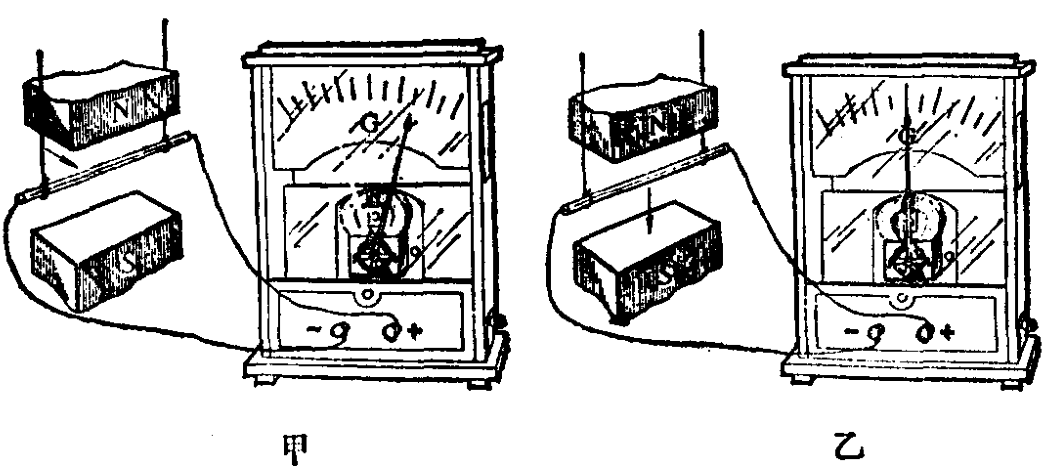
\includegraphics[width=0.7\textwidth]{../pic/czwl2-ch10-45}
    \caption{}\label{fig:10-45}
\end{figure}

在磁场中悬挂一根直导体,把导体的两端分别连接在电流表的两个接线柱上,组成一个闭合电路(图 \ref{fig:10-45})。
导体不动时,电流表的指针不发生偏转,表明导体中没有电流。
如果让导体在磁场中向前或向后运动切割磁力线,电流表的指针就发生偏转,表明导体中有了电流(图 \ref{fig:10-45} 甲)。
我们再让导体在磁场中向下或向上运动,不切割磁力线,可以看到电流表的指针不动,表明导体中没有电流(图 \ref{fig:10-45} 乙)。
可见,\textbf{闭合电路的一部分导体在磁场里做切割磁力线的运动时,导体中就会产生电流}。
这种现象叫做\textbf{电磁感应},产生的电流叫做\textbf{感生电流}。

\begin{wrapfigure}{r}{6cm}
    \centering
    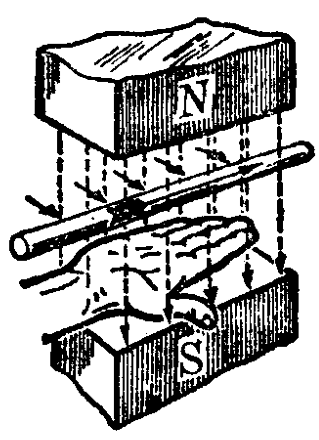
\includegraphics[width=5cm]{../pic/czwl2-ch10-46}
    \caption{}\label{fig:10-46}
\end{wrapfigure}

如果导体不是闭合的,即使做切割磁力线的运动,也不会产生感生电流,只是在导体两端产生感生电压。

在图 \ref{fig:10-45} 的实验中,当闭合电路的一部分导体做切割磁力线运动的方向改变时,电流表指针的偏转方向也改变。
可见导体中感生电流的方向跟导体运动的方向有关系。
如果导体切割磁力线运动的方向不变,而把两个磁极对调过来,使磁力线的方向改变,感生电流的方向也要改变。
可见导体中感生电流的方向还跟磁力线的方向有关系。

感生电流的方向和导体运动的方向、磁力线的方向之间的关系,可以用右手定则来判定:
伸开右手,使大拇指跟其余四个手指垂直,并且都跟手掌在一个平面内。
把右手放入磁场中,让磁力线垂直穿入手心,大拇指指向导体运动的方向,那么其余四个手指所指的方向
就是感生电流的方向(图 \ref{fig:10-46})。

我们使闭合电路的一部分导体做切割磁力线的运动时,用力移动导体做了功,消耗了机械能,
同时在导体中产生了感生电流,实现了由机械能向电能的转化。
所以在\CJKunderwave*{电磁感应现象里,机械能转化成电能}。



\section*{阅读材料}

\begin{wrapfigure}{r}{6cm}
    \centering
    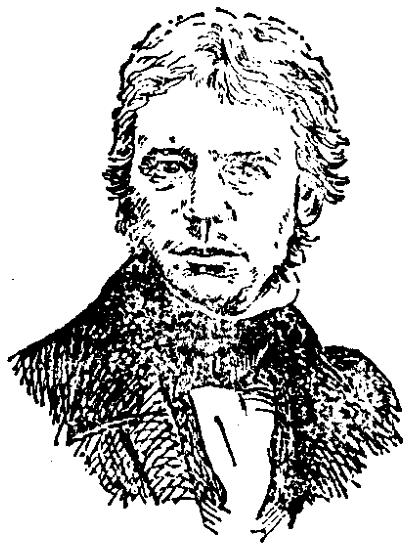
\includegraphics[width=5cm]{../pic/czwl2-ch10-faraday}
    \caption*{法拉第(1791 一1867)}\label{fig:10-faraday}
\end{wrapfigure}

法拉第是著名的英国物理学家和化学家。
他发现了电磁感应现象,提出了电场和磁场的概念,发现了电解定律等。
他的很多成就都是很重要、带根本性的。

法拉第出身于一个铁匠家庭,家境贫寒,没有念多少书,十三岁就开始当报童、学徒。
他热爱科学,立志献身于科学事业。
在做图书装订工期间,他就阅读了大量科学书籍,并在自己家里搞了一个小实验室。
后来,他到英国皇家学院担任实验室助理,由于勤奋好学,很快就能独立做实验。
法拉第是一个伟大的实验物理学家。他的许多重要发现都是通过实验获得的。
法拉第同时又是一个伟大的科学思想家,他总是力图搞清楚物理现象的本质,
他由于刻苦思索而具有深刻的洞察力,电场和磁场的提出可以看作是他作为科学思想家的重大成就。

法拉第对社会作出了巨大的贡献,人们给予他崇高的地位和荣誉,但他并不看重这些。
他拒绝了制造商们的高价聘请,专心致力于科学研究。他出身贫苦,成名以后仍然热爱贫苦人民。
他在皇家学会里还发起专门向青少年普及科学知识的讲座,自己坚持讲了十九年。
法拉第的高尚的道德品质,也同他在科学上的成就一样,受到人们的称颂。

